\chapter{Compressor maps mathematical models}
\label[secinapp]{chap:cp-maps-models}
\resetallacronyms

\section{History}
\label[secinapp]{sec:math-model-cp-history}

The development of the compression unit has started in 2002 with the
feasibility study presented by \citet{schiffmann-godat-2002a}. The
study attests of the feasibility of a twin-stage radial flow
compressor with a 19.8mm and a 18.4mm-impeller rotating at 240 krpm
with a total shaft power of 6kW \citep[p. 12 \&
14]{schiffmann-godat-2002a}. The compression unit would be designed
for domestic heating applications. From 2004 to 2008,
\citet{schiffmann-2008a} has developed a single-stage compression
unit of 3 kW with a 20mm-impeller. From 2008 to 2012, the company
Fischer Precise Engineering Solutions AG\footnotep{Fischer Precise
  Engineering Solutions AG is a Swiss company based in
  Herzogenbuchsee, in Switzerland,
  \url{http://www.fischerspindle.com/facilities/fischer-engineering-solutions-ag/}.}
has been pushing the development of the single-stage unit to a
twin-stage unit using the preliminary design and prototype developed
by \citet{schiffmann-2008a}. During those 4 years, 4 design families
have been issued\footnotep{Details about the design families are given
  in \cpref{sec:bwp-history}.}. A working prototype, the unit
\textit{cp105} from the \textit{evo4} design family, has successfully
be tested in May 2012 in the \AWP{}. An other prototype of the same
design family, the unit \textit{cp101}, has been used in October 2013
in the \BWP{}. Since 2013, the development of the compression unit has
lifted off and the compression units are now industrial products.

\section{Why a mathematical model of the compression maps?}
\label[secinapp]{sec:math-model-why}

In order to integrate those compression units, now technically ready,
in heat pumps, the integrator needs to know how to control them in
interaction with the controls of the thermodynamic
cycle. \Cref{sec:awp-issue-control-indus},
p.\,\pageref{sec:awp-issue-control-indus}, suggests notably that using
a model-based approach to control the heat pump could be the way to
control the cycle properly and steadily. In order to include a
model-based control in the heat pump controller, the integrator needs
to include the maps of the compression stages in the model. The
compressor maps are predicted with a physical model of the compressor,
during the design phase, then the maps are determined by testing and
measurements with each compression unit manufactured, as the maps
depend on the geometrical parameters of the compression units, which
slightly change with each unit. Integrating those maps in the
controller is not convenient, as that implies to fill the controller
with the points of the maps and to interpolate between the points. An
other approach is to offer a mathematical model of the compressor maps
and fit the model parameters with an identification test of the
compression unit. The advantages are:

\begin{itemize}
\item The testing and measurement phase of each compression unit is a
  lot shorter, since a few points allow to identify the parameters of
  the model.
\item The controller might need less computation power and memory to do the job.
\item In the future, the compression unit could even identify its
  model parameters itself with a self-learning phase.
\end{itemize}

\section{Mathematical model of a compression map}
\label[secinapp]{sec:math-model-model}
\label[secinapp]{sec:op-domain}

A compressor map is a diagram which describes the link between the
pressure ratio developed by the compressor and its mass flow rate, for
each rotor speed. There is a compressor map per inlet conditions,
being characterized by an inlet temperature and an inlet pressure. The
compressor maps can be made dimensionless using Mach
numbers \citep{Haugwitz-2002a}, as a Mach number is characterized
notably by the pressure and the temperature of the fluid. If the map
becomes dimensionless, one map only characterizes all the possible
inlet conditions.

\begin{table}[htbp]
  \centering
  \begin{tabular}{llll}
    \toprule
    Map & Abscissa & Ordinate & Parametric speed \\
    \midrule
    Classical map & Mass flow rate $\dot{M}$ & Pressure ratio $\Pi$ & Rotor speed $N$ \\
    Dimensionless map & Inlet Mach number $\mathcal{M}_{cp,in}$
    & Pressure ratio $\Pi$ & Impeller tip Mach number $\mathcal{M}_{cp,tip}$ \\
    \bottomrule
  \end{tabular}
  \caption{Characteristics of the classical and the dimensionless compressor maps}
  \label{tab:maps-diffs}
\end{table}

\subsection{Modeling of the compressor iso-speed curves}

The iso-speed curves are modeled using Lamé equations, also called
super-ellipses equations \citep{Haugwitz-2002a,Haugwitz-2003a}. The
generic form of a Lamé equation is given in
\cref{eq:lame-generic}. The specific form used in this thesis work and
described in \cref{eq:lame-specific} uses the Lamé curves and applies
them with scaled values, and with rotated coordinates, in order to
decrease the prediction errors.

\begin{flalign}
  & \left|\dfrac{x}{a}\right|^z + \left|\dfrac{y}{b}\right|^z = 1
  \label{eq:lame-generic} \\
  & \left|\dfrac{\mathcal{M}_{cp,\,in,\,scaled,\,rotated}}{a}\right|^z + \left|\dfrac{\Pi,\,scaled,\,rotated}{b}\right|^z =
  1 \label{eq:lame-specific}
\end{flalign}

The parameters a, b, and z are modeled using quadratic polynomials, as
described in \cref{eq:a,eq:b,eq:z}.

\begin{flalign}
  & a = \sum_{i=0}^{2}a_i\, \mathcal{M}_{cp,\,tip,\,scaled}^i \label{eq:a} \\
  & b = \sum_{i=0}^{2}b_i\,
  \mathcal{M}_{cp,\,tip,\,scaled}^i \label{eq:b}\\
  & z = \sum_{i=0}^{2}z_i\, \mathcal{M}_{cp,\,tip,\,scaled}^i +
  \kappa_{cp}\,sum_{i=0}^{2}z_i\, \mathcal{M}_{cp,\,tip,\,scaled}^i
  \, \left( \rho_{cp,\,in\,scaled} - \dfrac{1}{2} \right) \label{eq:z}
\end{flalign}

The coefficients $a_{i}$, $b_{i}$, $z_{i}$ are fitted on the
compressor map resulting from physical modeling or from measurements.

The inlet Mach Number $\mathcal{M}_{cp,\,in}$ and tip Mach Number
$\mathcal{M}_{cp,\,tip}$ \footnotep{The tip Mach number is a
  characteristic value, an indicator, and does not formally defines a
  physical phenomenon, as the number is calculated from the impeller
  geometry and gas characteristics. It is consequently abusive to call
  it a Mach Number. It is called this way for the sake of simplicity.}
are defined in \cref{eq:Mcpin} and \cref{eq:Mcptip}.

\begin{flalign}
  & \mathcal{M}_{cp,\,in} = \dfrac{C_{cp,\,in}}{a_{cp,\,in}} =
  \dfrac{\dot{M}_{cp}}{a_{cp,\,in}\,\rho_{cp,\,in}\,A_{cp,\,in}} \label{eq:Mcpin} \\
  & \mathcal{M}_{cp,\,tip} = \dfrac{C_{cp,\,tip}}{a_{cp,\,in}} =
  \dfrac{\pi\,\varnothing_{cp,\,tip}\,N_{cp}}{60\,a_{cp,\,in}} \label{eq:Mcptip}
\end{flalign}

The inlet Mach Number $\mathcal{M}_{cp,\,in}$ is the ratio of the
inlet fluid velocity $C_{cp,\,in}$ to the speed of sound in the fluid
at the compressor inlet $a_{cp,\,in}$. $\rho_{cp,\,in}$ is the fluid
density at the compressor inlet  and $A_{cp,\,in}$ is the section of
the compressor inlet.

The tip Mach Number $\mathcal{M}_{cp,\,tip}$ is the ratio of the
impeller rotation speed at the impeller tip $C_{cp,\,tip}$ to the
speed of sound in the fluid at the compressor inlet
$a_{cp,\,in}$. This Mach Number does not represent the real Mach
Number of the fluid flow at the outlet of the compressor and is
abusively called a Mach Number. This quantity allows a to couple the
rotation speed to physical properties of the fluid at the compressor inlet.

\subsection{Rotation of the coordinates}

\begin{flalign}
  & r = \sqrt{\mathcal{M}_{cp,\,in,\,scaled}^2 + PR_{scaled}^2} \label{eq:r}
\end{flalign}

\[
 \label{eq:phi}\phi =
  \begin{cases}
   0 & \text{if } \mathcal{M}_{cp,\,in,\,scaled}=0 \text{ and }
   PR_{scaled}=0 \\
   \arcsin\left(\dfrac{PR_{scaled}}{r}\right) & \text{if }
   \mathcal{M}_{cp,\,in,\,scaled} \geq 0 \\
   -\arcsin\left(\dfrac{PR_{scaled}}{r}\right) + \pi & \text{if }
   \mathcal{M}_{cp,\,in,\,scaled} < 0
  \end{cases}
\]

\begin{flalign}
  & \Psi = \phi - \theta_{cp} \label{eq:psi} \\
  & \mathcal{M}_{cp,\,in,\,scaled,\,rotated} = r\,\cos(\Psi) \\
  & PR_{scaled,\,rotated} = r\,\sin(\Psi)
\end{flalign}

The coefficients $\theta_{cp}$ and $\kappa_{cp}$ are fitted on the
compressor map resulting from physical modeling or from measurements.

\subsection{Modeling of the isentropic efficiency}

The isentropic efficiency can be modeled also with the inlet an tip
Mach numbers. The curves are modeled with degree-four polynomials and
values are scaled in order to obtain better correlations. The
coefficient of those polynomials are modeled with polynomials at
degrees ranging from 2 to 6, as described in
\cref{eq:eta_s_model,eq:d}.

\begin{flalign}
  & \eta_{cp,\,s,\,scaled} = \sum_{j=0}^{4}d_j\,
  \mathcal{M}_{cp,\,in,\,scaled}^i \label{eq:eta_s_model} \\
  & d_j = \sum_{i=0}^{2 to 6}d_{ji}\,
  \mathcal{M}_{cp,\,in,\,scaled}^i \label{eq:d}
\end{flalign}

The coefficients $d_{ji}$ are fitted on the compressor map resulting
from physical modeling or from measurements.

\section{Errors of the correlations}

The correlations are used to predict the mass flow rate, deduced from
the inlet Mach number, from the measured pressure
ratio. Unfortunately, at low mass flow rates, the compressor iso-speed
curves become almost flat, which means that prediction of low mass
flow rates with any correlation is a difficult operation. In order to
keep the the errors in acceptable ranges, a rotation of the
coordinates is performed. A two-objective optimization is run on the
fitted parameters described in the sections above in order to keep the
average error over the whole map and maximum error in acceptable
ranges. From the Pareto curve obtained with the optimization, a
solution is selected. The author recommends to give more weight in the
decision process to low average errors, as the compressor is likely to
work most of the time in low error areas. Indeed, the domain where the
prediction is inaccurate is very close to the surge
line.

\begin{figure}[htbp]
  \centering \subfloat[Error map for the first compression
  stage]{\label{fig:cp1-error-map} 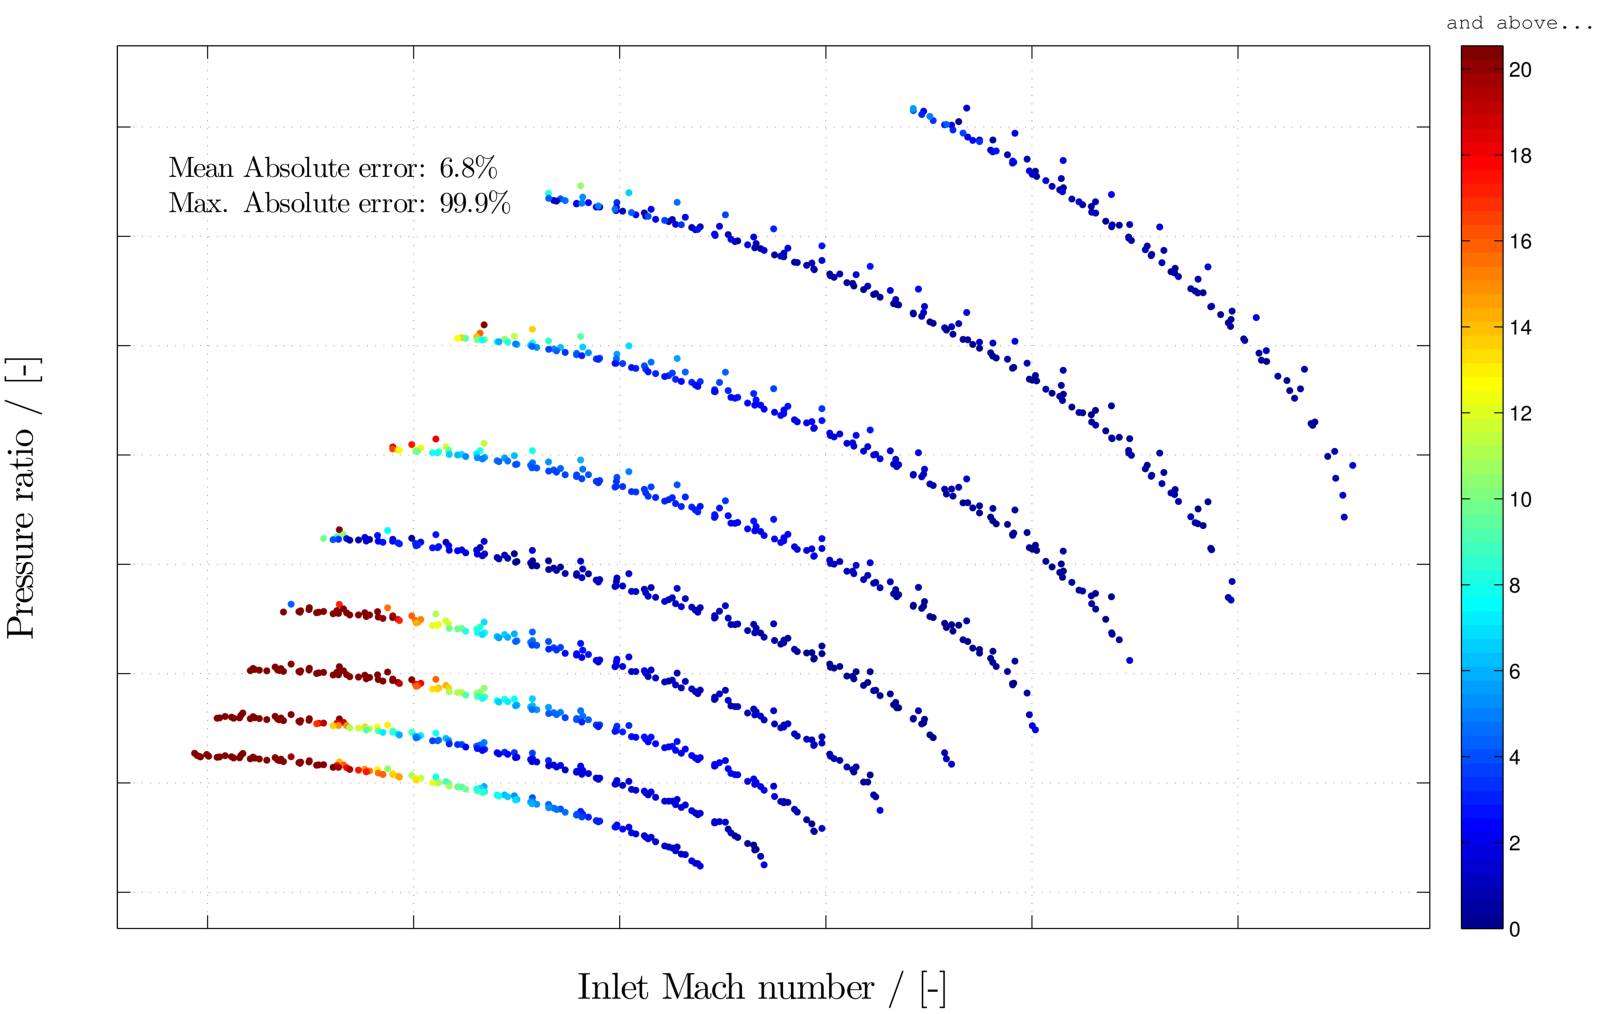
\includegraphics[height=7.2cm]{cp1_lame_gal3_poly224_errormap-noaxis}}
  \subfloat[Occurrences of the errors]{\label{fig:cp1-error-occurrence}
    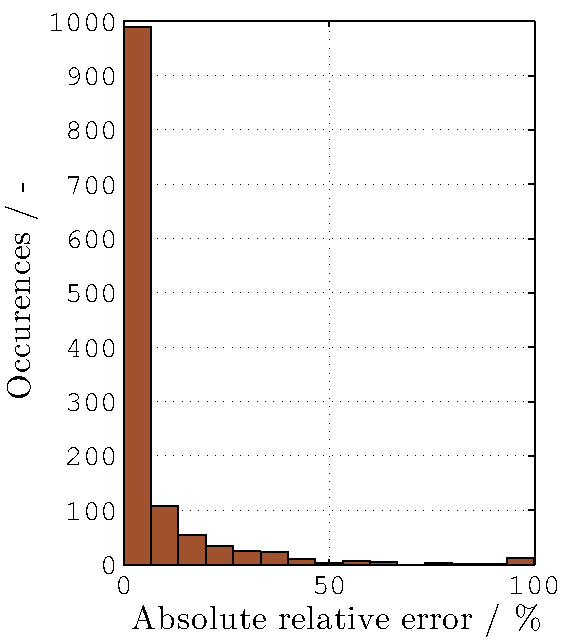
\includegraphics[height=4.5cm]{cp1_lame_gal3_poly224_errorhist}} \\
  \subfloat[Correlation curves for the first compression stage]{\label{fig:cp1-error-correl-curves}
    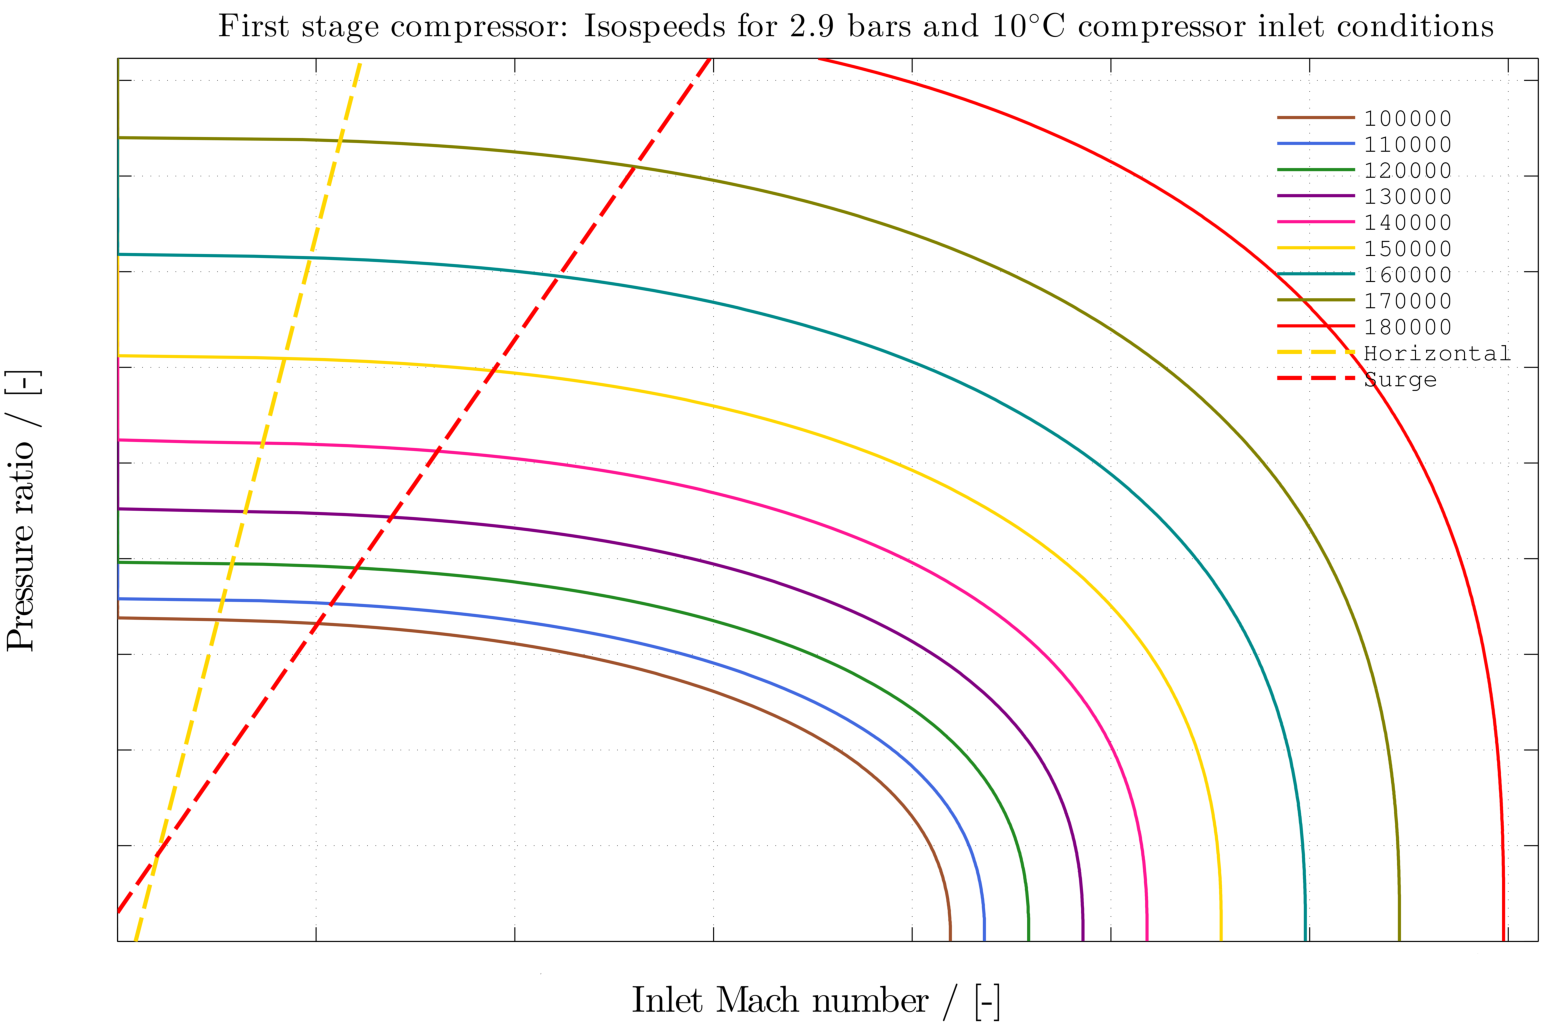
\includegraphics[height=4.5cm]{cp1_lame_gal3_poly224_curves-noaxis}}
  \hspace{2em} \subfloat[Coefficients of the correlations (first
  stage)]{\label{fig:cp1-error-correl-coefs}
    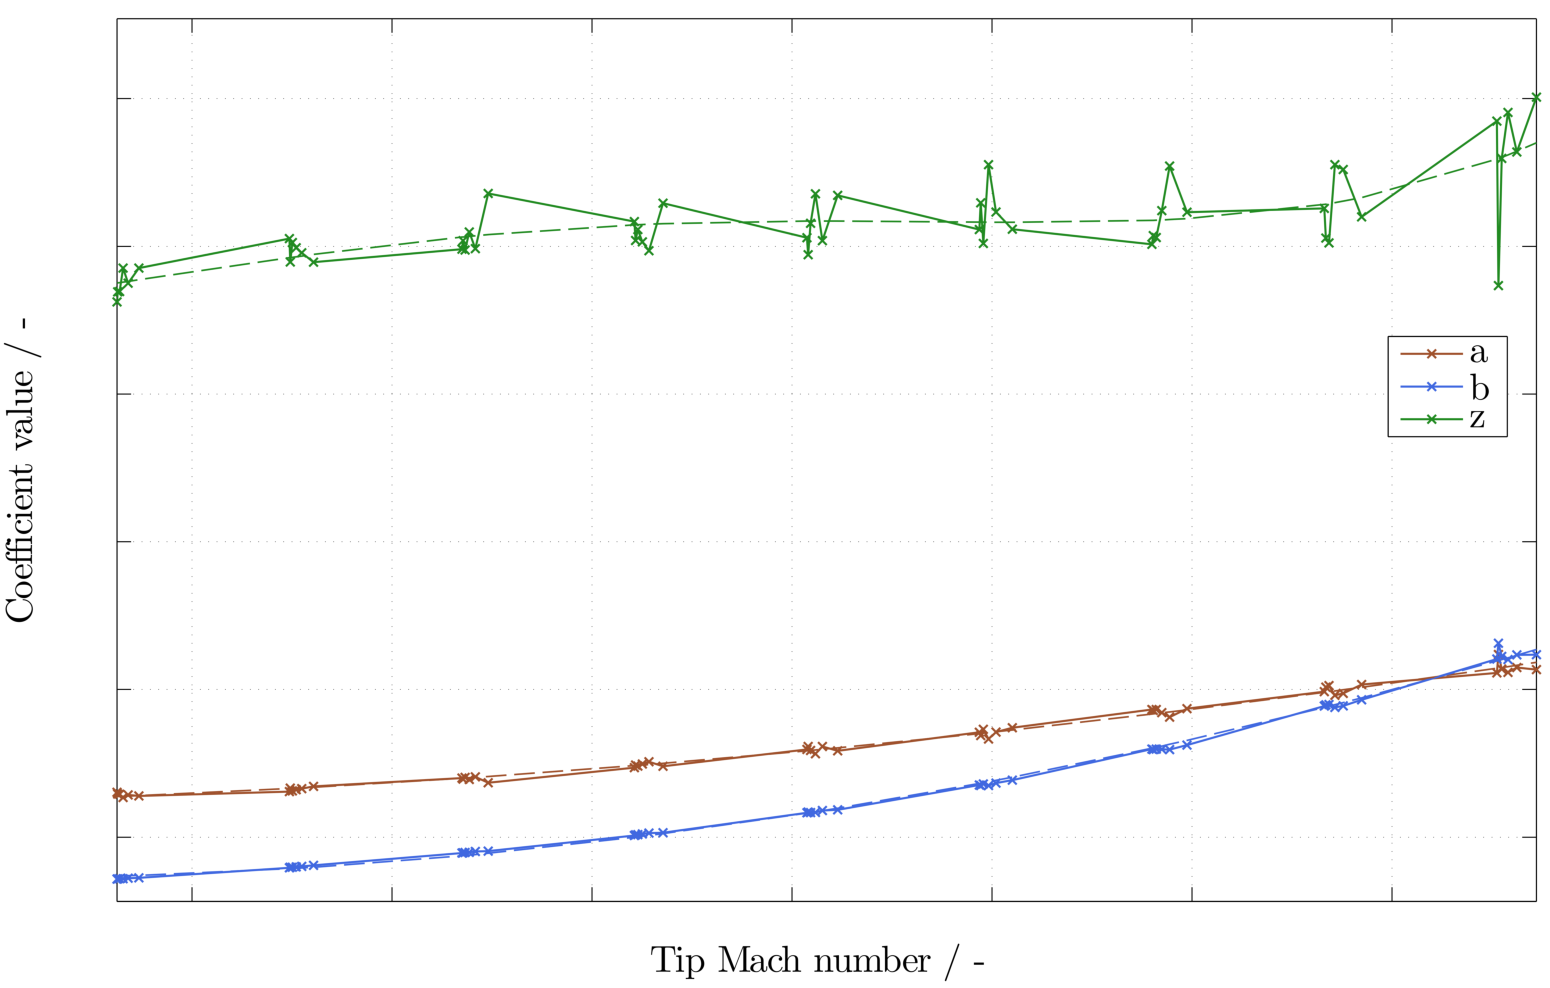
\includegraphics[height=4.5cm]{cp1_lame_gal3_poly224_params-noaxis}}
  \caption[Errors in the first compression stage map
  correlations]{Errors in the first compression stage map
    correlations. The axis have been removed due to confidentiality
    issues.}
  \label{fig:cp1-errors}
\end{figure}

\begin{figure}[htbp]
  \centering \subfloat[Error map for the second compression stage]{\label{fig:cp2-error-map}
    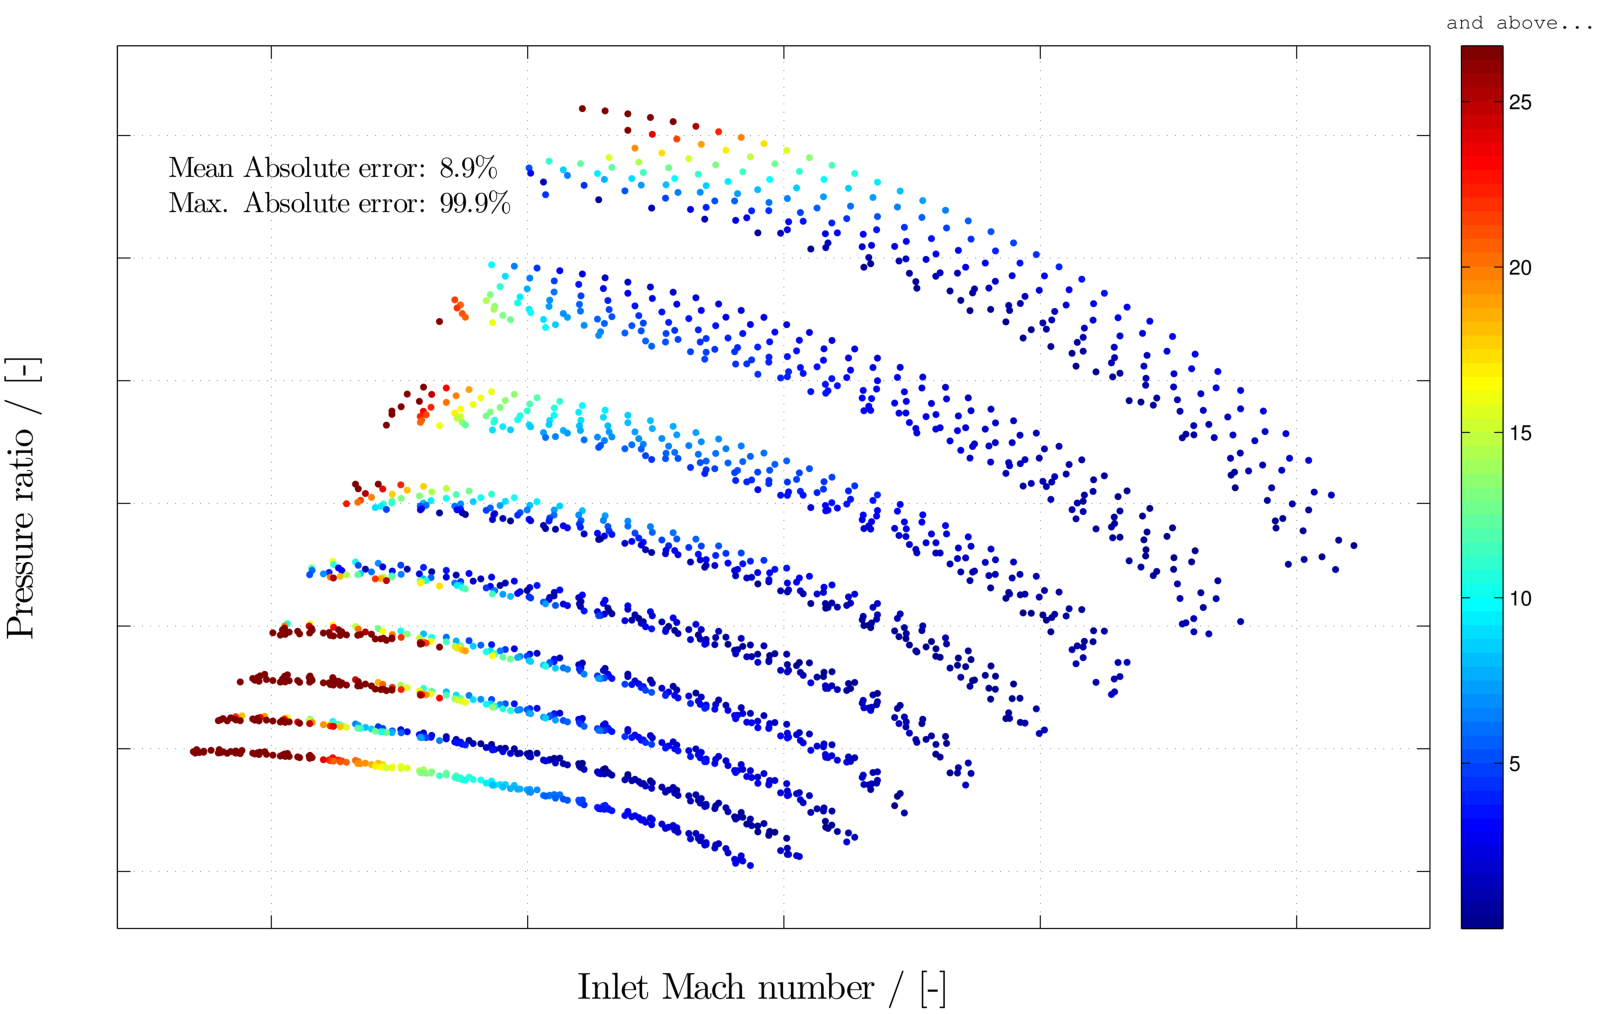
\includegraphics[height=7.2cm]{cp2_lame_gal3_poly224_errormap-noaxis}}
  \subfloat[Occurrences of the errors]{\label{fig:cp2-error-occurrence}
    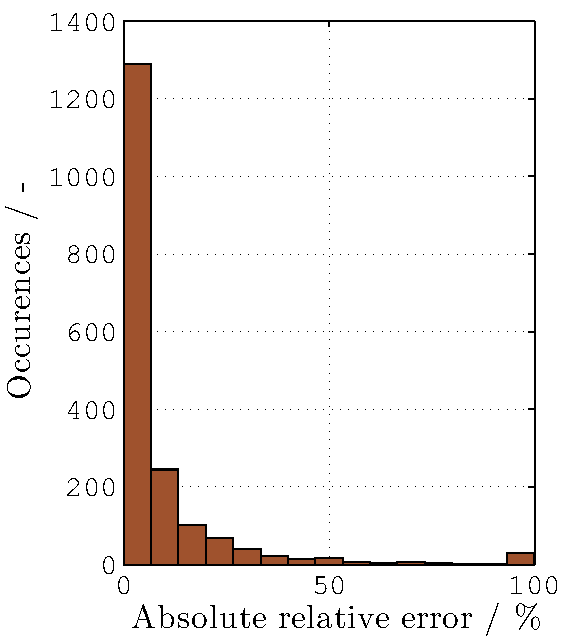
\includegraphics[height=4.5cm]{cp2_lame_gal3_poly224_errorhist}} \\
  \subfloat[Correlation curves for the second compression
  stage]{\label{fig:cp2-error-correl-curves}
    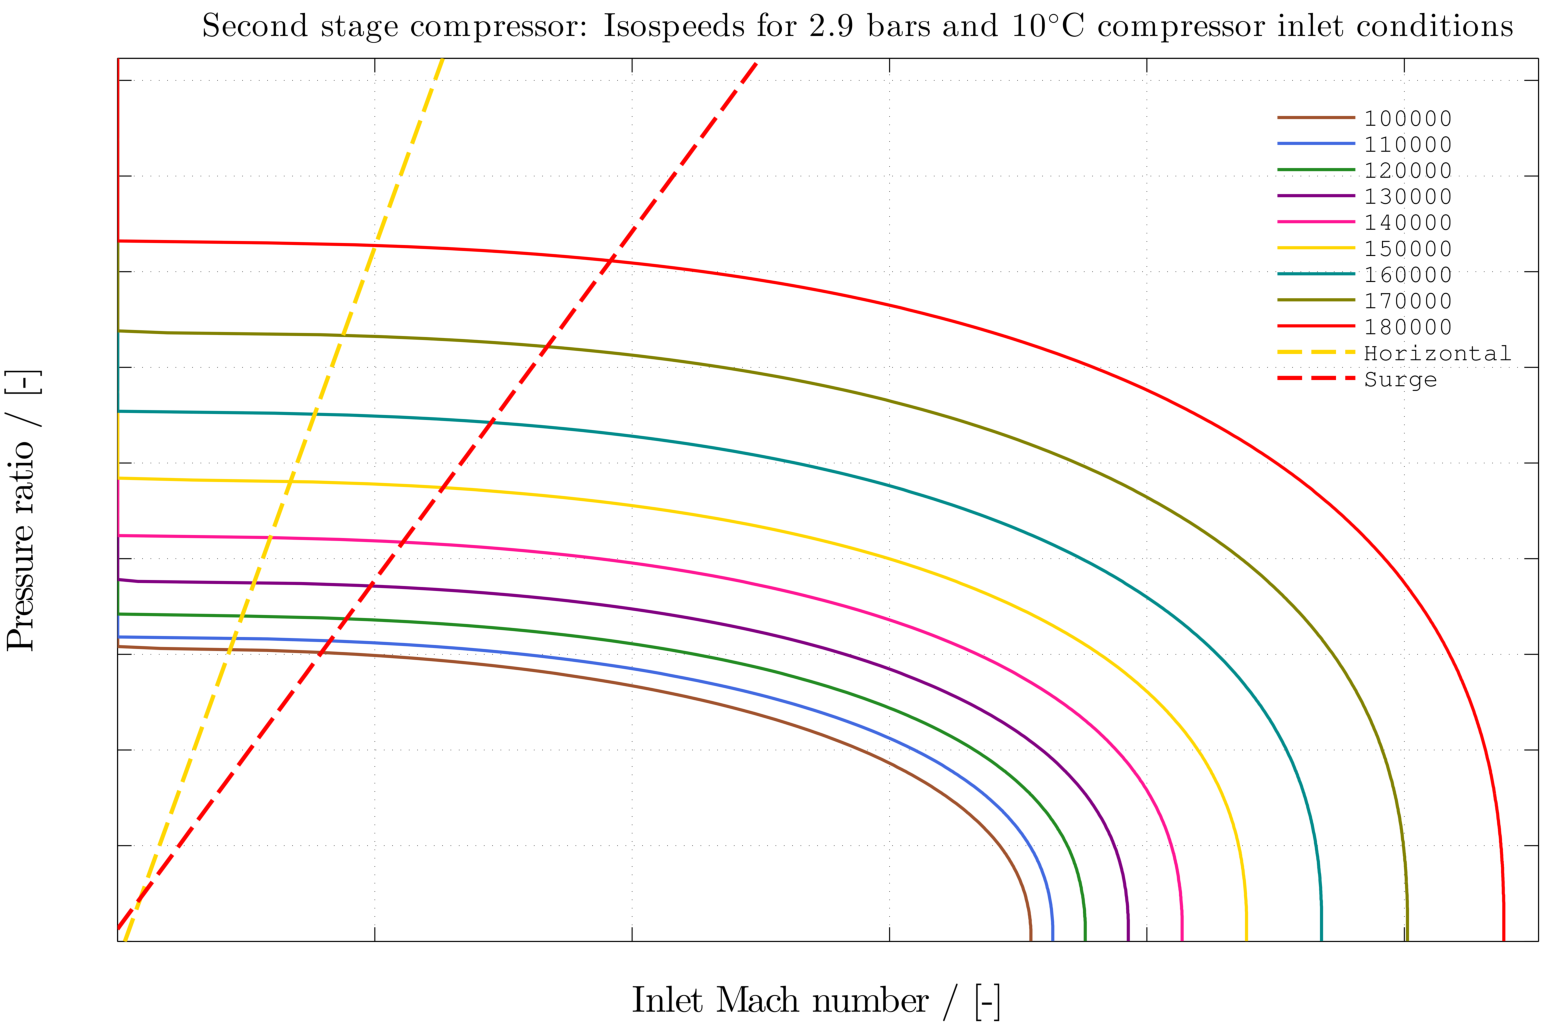
\includegraphics[height=4.5cm]{cp2_lame_gal3_poly224_curves-noaxis}}
  \hspace{2em}
  \subfloat[Coefficients of the correlations (second stage)]{\label{fig:cp2-error-correl-coefs}
    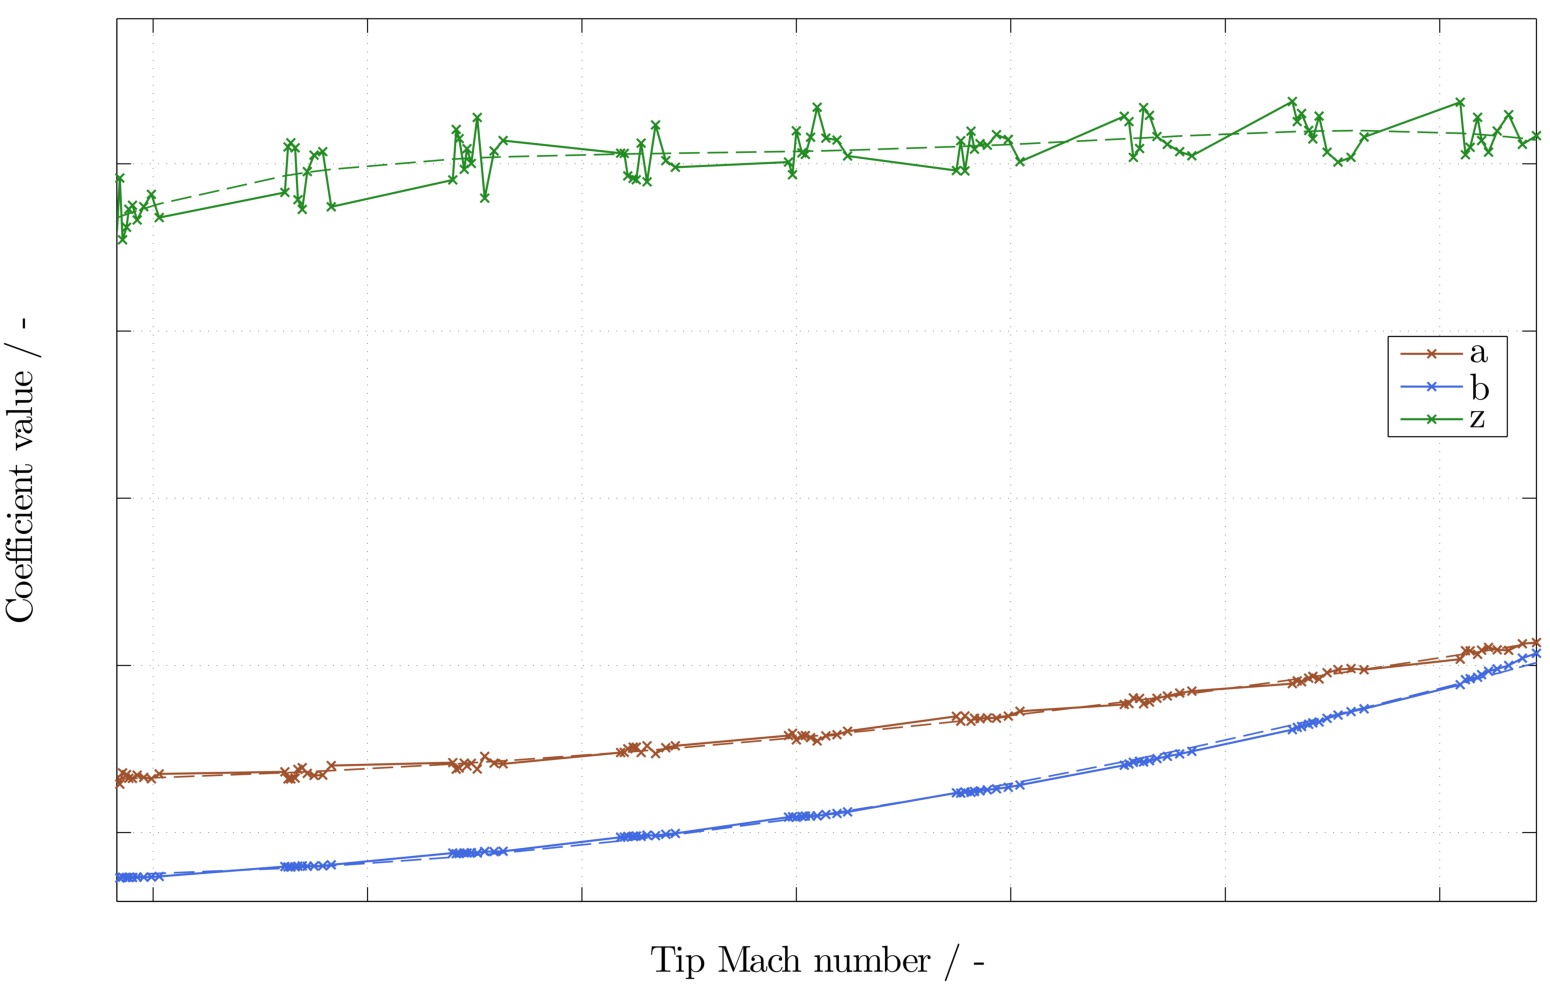
\includegraphics[height=4.5cm]{cp2_lame_gal3_poly224_params-noaxis}}
  \caption[Errors in the second compression stage map
  correlations]{Errors in the second compression stage map
    correlations. The axis have been removed due to confidentiality
    issues.}
  \label{fig:cp2-errors}
\end{figure}

\FloatBarrier
\bibliographystyle{plainnat}
\bibliography{main}
\label[secinapp]{sec:math-model-refs}